\documentclass[a4, landscape] {article}
\usepackage{tikz}
\begin{document}

% \begin{tikzpicture}
 
 
 % Vakio r -kaaret
 % \foreach \r in {0.1,0.6,...,2.0}{
 %     \draw[ultra thick, red!75!black] (\r,0) arc (0:72:\r);
%  }
  
 % Vakio fii -viivat
 % Päätepisteet
%  \coordinate (A) at (2,0);
 % \coordinate (B) at (1.61 , 1.17 );
%  \coordinate (C) at (0.61 , 1.90 );
  %\coordinate (D) at (-0.61, 1.90 );
  %\coordinate (E) at (-1.61, 1.17 );
  %\coordinate (F) at (-2.0 , 0    );
  %\coordinate (G) at (-1.61, -1.17);
  %\coordinate (H) at (-0.61, -1.90);
 % \coordinate (I) at (0.61 , -1.90);
 % \coordinate (J) at (1.61 , -1.17);

%  \foreach \point in {A, B, C}{% D, E, F, G, H, I, J}{
%      \draw[ultra thick, green!50!black] (0,0) -- (\point);
%      } 
      
 
 % Origo
 %\draw[fill] (0,0) circle (2pt); 
  % jokin piste   
%  \draw[fill] (1.29,0.945) circle (4pt);
 
% \end{tikzpicture}
 
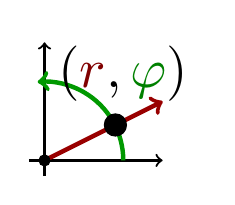
\begin{tikzpicture}

\draw[thick, ->] (-.2,0) -- (1.5,0); 
\draw[thick, ->] (0,-.2) -- (0,1.5); 

%\draw[red!80!black, ->] (0,0) -- (2.2,0.5); 
\draw[ultra thick, red!60!black, ->] (0,0) -- (1.5,.75); 
%\draw[red!80!black, ->] (0,0) -- (0.7,2.2); 
%\draw[green!80!black, ->] (0.75,0) arc (0:100:0.75);
\draw[ultra thick, green!60!black, ->] (1,0) arc (0:95:1);
\draw[fill] (.9, .45) circle (4pt);

\draw[fill] (0,0) coordinate (O) circle (2pt);

\node[scale=2] at (1, 1.1) {$(\textcolor{red!50!black}r,\textcolor{green!50!black}\varphi)$};

%\node at (.5,-0.2) {Napa};

\end{tikzpicture}

%\begin{tikzpicture}

%\draw[fill, orange!15] (-.5,-.5) -- (-.5,.5) -- (.5,.5) -- (.5,-.5) -- cycle;
%\node at (0, 0) {$(\textcolor{red!75!black}r,\textcolor{green!75!black}\varphi)$};

%\end{tikzpicture}

%\begin{tikzpicture}

%\draw[fill, blue!15] (-.5,-.5) -- (-.5,.5) -- (.5,.5) -- (.5,-.5) -- cycle;
%\node at (0, 0) {$(\textcolor{red!75!black}r,\textcolor{green!75!black}\varphi)$};

%\end{tikzpicture} 

%\begin{tikzpicture}

%\draw[gray, ->]( 0,0,0) coordinate (O) -- (4,0,0) coordinate (x);
%\draw[gray, ->] (O) -- (0,4,0) coordinate (y);
%\draw[gray, ->] (O) -- (0,0,4) coordinate (z);

%\draw[red] (0,0,0) circle (2cm);

%\draw[black] plot [smooth cycle, tension=1] coordinates {(1,3,0) (0,3,1) (-1,3,0) (0,3,-1)};
%\draw[black] plot [smooth cycle, tension=1] coordinates {(1,0,0) (0,0,1) (-1,0,0) (0,0,-1)};
%\draw (-1,0,0) -- (-1,3,0) ;
%\draw (1,0,0) -- (1,3,0) ;

%\end{tikzpicture}

\end{document}